\documentclass{article}

\usepackage[portuguese]{babel}
\usepackage[utf8]{inputenc}
\usepackage{amsmath}
\usepackage{graphicx}
\usepackage{fancyvrb}
\usepackage{fullpage}
\usepackage{float}
\usepackage{amsmath}
\usepackage{color}
\usepackage{spverbatim}


\definecolor{ogreen}{RGB}{60,128,49}

\restylefloat{table}

\title{%
  Estruturas Discretas - Primeiro Trabalho\\
  \large Prof. Marcus Vinicius S. Poggi de Aragão\\
  Período de 2017.1}

\author{Gabriel Barbosa Diniz\\1511211 \and Lucas Rodrigues\\1510848 \and Mateus Ribeiro de Castro\\1213068}

\date{\today}

\begin{document}
\maketitle

\textbf{Observação}: Os códigos fontes dos algoritmos referentes aos teoremas provados seguirá em anexo em um arquivo Jupyter Notebook para melhor entendimento, compilação, execução, testes, etc.

\section{Primeira Questão (Teorema 1)}

Dado o Teorema 1 e sua prova indutiva, deseja-se um algoritmo que, dados $x$, $y$ e $n$, determine o quociente descrito. Também se deseja os testes dos algoritmos para os vários valores de $x$, $y$ e $n$.\\

\textbf{Teorema 1} ($n$): $x^n - y^n$ é divisível por $x-y$ para quaisquer $x$ e $y$ inteiros e todos os valores de $n$ inteiros e maiores do que zero.\\

Com as condições mencionadas acima, obtemos o seguinte quociente: $\frac{x^n - y^n}{x-y}$, e a partir do caso base, sabemos que para $n = 1$, o quociente é igual a 1. Também diretamente da argumentação fornecida, tem-se que:

\begin{gather}
x^{n+1} - y^{n+1} = q_{n+1} * (x - y) \\
q_{n+1} = (x^n + y * q_n)
\end{gather}

E assim então podemos, através da prova indutiva fornecida no enunciado, derivar um algoritmo correspondente que prove este teorema...\\

\textbf{Implementação em Python}:

{\color{blue}
\begin{verbatim}
def coeficiente(x, y, n):
    #Checa se n é positivo e maior que zero
    if(n <= 0):
        print("Parametros invalidos, n menor ou igual a zero!\n")
        return -1
    #Checa se estamos trabalhando com o caso base
    if(n == 1):
        return 1
    #CASO BASE: q1 = 1
    q = 1
    #Será um método iterativo, processando até n
    for i in range(0, n-1):
        q = m.pow(x, (i+1)) + y * q
    return q
\end{verbatim}
}

\pagebreak

\textbf{Testes do Algoritmo}: Os testes se encontram no arquivo Jupyter Notebook juntamente com o gráfico que corresponde ao tempo de execução. Como função de teste, foi implementado uma função em Python que exibe na tela cada caso de teste, tendo chamado a função que obtém o coeficiente. Valores para $x$, $y$ e $n$ foram aleatoriamente escolhidos enquanto o valor de $i$ permanecia em ordem. A imagem abaixo demonstra os tempos de execução em formato de gráfico para melhor observação.

\begin{figure}[!htb]
\centering
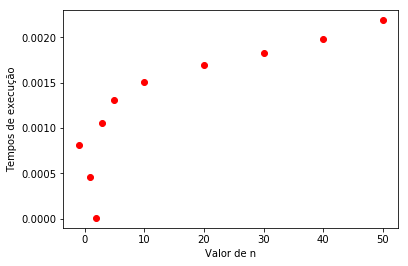
\includegraphics[scale=0.6]{GRAFICO.png}
\caption{Gráfico contendo os tempos de execução para diferentes valores para $n$.}
\end{figure}

\textbf{Conclusão}: Observando o gráfico dos testes executados e através da própria análise do algoritmo utilizado, podemos constatar que o parâmetro $n$ exerce grande influência na execução, ou seja, com a variação de $n$ podemos ver que há uma progressão linear temporal e a complexidade em função de $n$ é linear.\\

\textbf{Observação Importante}: Por questão de eficiência, o algoritmo poderia também ser realizado de forma recursiva, porém decidimos por fazer pela forma iterativa. Caso fosse pela forma recursiva teríamos o seguinte algoritmo com os seguintes tempos de execução:\\

\textbf{Implementação Recursiva em Python}:

{\color{red}
\begin{verbatim}
def quociente(x, y, n):
    if n == 1:
        return 1
    return x ** (n-1) + y * quociente(x, y, n-1)
\end{verbatim}
}

\begin{table}[H]
\centering
\begin{tabular}{l|l|l|l|l|l}
$x$ & $y$ & $n$ & Execuções & Tempo Total & Tempo/Execução \\\hline
2 & 2 & 1 & 18900000 & 5.006 s & 0.000265 ms \\
2 & 2 & 2 & 5600000 & 5.074 s & 0.000906 ms \\
2 & 2 & 3 & 2900000 & 5.136 s & 0.001771 ms \\
2 & 2 & 4 & 2100000 & 5.190 s & 0.002471 ms \\
2 & 2 & 5 & 1600000 & 5.176 s & 0.003235 ms \\
2 & 2 & 6 & 1400000 & 5.255 s & 0.003754 ms \\
2 & 2 & 7 & 1200000 & 5.373 s & 0.004477 ms \\
2 & 2 & 8 & 1000000 & 5.285 s & 0.005285 ms \\
2 & 2 & 9 & 900000 & 5.346 s & 0.005940 ms \\
2 & 2 & 10 & 800000 & 5.476 s & 0.006845 ms \\
\end{tabular}
\end{table}

\pagebreak

\section{Segunda Questão (Teorema 2)}

\textbf{Teorema 2} ($k$): Seja $G = (V, E)$ um grafo denso. Sabe-se encontrar um caminho Hamiltoniano em $G$ onde $|V| >= 3$.\\

\textbf{Caso base}: Temos como teorema de caso base o Grafo completo, pois todo grafo completo com pelo menos $3$ vértices contém um ciclo Hamiltoniano. Basta colocar os vértices em uma ordem qualquer e conectá-los em um ciclo. Validando então o caso base.\\

\textbf{Hipótese de Indução}: Sabe-se encontrar um ciclo Hamiltoniano em um grafo com as especificações especificadas acima e com o número de arestas maior ou igual a $k$.\\

\textbf{Passo indutivo}: Deve-se provar que sabe-se encontrar um ciclo Hamiltoniano em um grafo com $k-1$ arestas que satisfaça as condições do problema. $G = (V,E)$ será esse grafo com $k-1$ arestas. Pegando um par de vértices não adjacentes $v$ e $w$ em $G$ e considerar o grafo $G$’ que é igual a $G$ mas com $v$ e $w$ conectados. Pela hipótese de indução sabe-se encontrar um ciclo Hamiltoniano com $k$ arestas. Se a aresta $(v,w)$ não está no ciclo então esse ciclo está presente em $G$, senão (sabendo que a soma das arestas em $v$ e $w$ será no mínimo $n$) toma-se v como primeiro ($v_1$) e $w$ como último ($v_n$) vértices no ciclo encontrado em $G$’ e toma dois vértices vizinhos ($v_i$ e $v_i+1$) tal que o primeiro ($v_i$) esteja ligado a $w$ e o segundo ($v_i+1$) a $v$. Dessa forma o novo ciclo é formado partindo de $v$ para $v_i+1$, segue o caminho até $w$, vai para $v_i$ e então percorre o caminho até $v$ provando o teorema.\\

E assim podemos então, através do passo indutivo, obter um algoritmo que prove este teoremas de acordo com as devidas instâncias disponibilizadas para realização de testes e desempenho da CPU no processamento!\\

\textbf{Implementação em Python}:

{\color{blue}
\begin{verbatim}
#CODIGO
\end{verbatim}
}

\pagebreak

\section{Terceira Questão (Teorema 3)}

\textbf{Teorema 3} ($k$): Em um campeoknato com $k = 2^k$ equipes, sabe-se construir as $2^k - 1$ rodadas de $2^{k - 1}$ jogos onde cada equipe enfrenta uma equipe diferente em cada rodada.\\

\textbf{Intuição}: Em cada rodada, cada equipe participará de um só jogo, e como cada jogo envolve duas equipes, cada rodada terá $n/2 = 2^{k-1}$ jogos. Como cada equipe só joga com uma outra por rodada, deverão existir $n-1 = 2^k -1$ rodadas para que cada equipe possa jogar com todas as outras.\\

\textbf{Prova}: feita por indução matemática usando $k$ como parâmetro de indução. As equipes serão numeradas de $e_1$ até $e_{2^k} = e_n$.\\

\textbf{Caso base} ($k = 1$): temos $n = 2$. Haverá $n-1 = 1$ rodada, com $n/2 = 1$ jogo. Esse jogo é $[e_1, e_2]$.\\

\textbf{Passo indutivo}: podemos assumir que o teorema é válido para um certo $k$ (hipótese indutiva). Desejamos provar que, a partir disso, o teorema se torna válido para $k+1$. Nesse caso, existem $2^{k+1}$ equipes.\\

Divide-se as equipes em dois grupos, $A$ e $B$ de igual tamanho: $\{e_1, ..., e_{2^k}\}$ e $\{e_{2^k+1}, ..., e_{2^{k+1}}\}$. Cada grupo tem $2^k$ equipes. Neste primeiro momento, trataremos os dois grupos como dois torneios independentes e simultâneos. Pela hipótese indutiva, sabemos resolver esses dois problemas (idênticos), e geramos portanto dois torneios, cada um com $2^k - 1$ rodadas de $2^{k - 1}$. Como os torneios são simultâneos, a rodada 1 do torneio $A$ ocorrerá ao mesmo tempo que a rodada 1 do torneio $B$, portanto, ao juntar essas rodadas, teremos $2^k$ jogos por rodada.\\

Após esse momento inicial, sabemos que cada equipe do grupo $A$ enfrentou todas as outras equipes de seu grupo. O mesmo vale para o grupo $B$. Resta, portanto, cada equipe do grupo $A$ enfrentar todas as equipes do grupo $B$, e vice-versa. Para fazer isso, teremos mais $2^k$ rodadas de $2^k$ jogos. Para gerar esses jogos, considere os conjuntos ordenados das equipes do grupo A e do grupo B.

\begin{gather}
a_1 = e_1 \\
a_2 = e_2 \\
... \\
a_{2^k} = e_{2^k}\end{gather}

\begin{gather}
b_1 = e_{2^k + 1} \\
b_2 = e_{2^k + 2} \\
... \\
b_{2^k} = e_{2^{k+1}}\end{gather}

A primeira rodada deste momento teremos os jogos $[a_1, b_1]$, $[a_2, b_2]$, ..., $[a_{2^k}, b_{2^k}]$.\\

Na segunda rodada, ocorrerá uma rotação nos times de $B$, de modo que o primeiro time de $A$ enfrentará o último time de $B$: $[a_1, b_{2^k}]$, $[a_2, b_1]$, ..., $[a_{2^k}, b_{2^k-1}]$.\\

Nas próximas rodadas, continuará ocorrendo essa rotação, até que na $2^k$-ésima rodada deste momento teremos: $[a_1, b_2]$, $[a_2, b_3]$, ..., $[a_{2^k-1}, b_{2^k}]$, $[a_{2^k}, b_1]$.\\

O total destes dois momentos é $(2^k -1) + (2^k) = 2^{k+1} - 1$ rodadas de $2^k$ jogos, o que está de acordo com o teorema.

\pagebreak

\textbf{Implementação em Python}:

{\color{ogreen}
\begin{verbatim}
# Start é um argumento opcional, usado pela recursão
# O retorno eh uma lista de rounds
# Um round eh uma lista de jogos
# Um jogo eh uma tupla indicando os dois times

def tournament(k, start = 1):
    # Caso base
    if k == 1:
        return [[(start, start+1)]]

    # MOMENTO 1 - divide em dois
    
    # Recursao
    t1 = tournament(k-1, start)
    t2 = tournament(k-1, 2**(k-1)+start)

    # Unir os rounds dos dois torneios
    t = []
    for i in range(len(t1)):
        t.append(t1[i] + t2[i])

    # MOMENTO 2 - ciclo
    
    # Geracao das listas de times
    times1 = range(start, 2**(k-1)+start)
    times2 = range(2**(k-1)+start, 2**(k)+start)
    
    # z vai ser a variavel que faz o ciclo
    for z in range(len(times1)):
        # Estamos em um round
        round = []
        for i in range(len(times1)):
            # Estamos em um par dentro do ciclo
            
            # index1 eh simplesmente i
            # index2 muda de modo a fazer o ciclo no segundo grupo
            index1 = i
            index2 = (i + z) % len(times2)

            game = (times1[index1], times2[index2])
            round.append(game)

        # Adicionamos esse round ao conjunto de rounds, t
        t.append(round)

    return t
\end{verbatim}
}

\pagebreak

\textbf{Exemplo}: Tendo $k = 3$, esse foi o resultado gerado pela implementação em Python:\\

\begin{table}[H]
\centering
\begin{tabular}{l|l|l|l|l}
Round & Game 01 & Game 02 & Game 03 & Game 04\\\hline
1.& 1 vs 2 & 3 vs 4 & 5 vs 6 & 7 vs 8\\
2.& 1 vs 3 & 2 vs 4 & 5 vs 7 & 6 vs 8\\
3.& 1 vs 4 & 2 vs 3 & 5 vs 8 & 6 vs 7\\
4.& 1 vs 5 & 2 vs 6 & 3 vs 7 & 4 vs 8\\
5.& 1 vs 6 & 2 vs 7 & 3 vs 8 & 4 vs 5\\
6.& 1 vs 7 & 2 vs 8 & 3 vs 5 & 4 vs 6\\
7.& 1 vs 8 & 2 vs 5 & 3 vs 6 & 4 vs 7\\
\end{tabular}
\end{table}

\textbf{Testes}: A tabela abaixo ilustra os resultados dos testes. O maior valor de $k$ para o qual o algoritmo gerou as rodadas foi 13.

\begin{table}[H]
\centering
\begin{tabular}{l|l|l|l}
$k$ & Execuções & Tempo Total & Tempo/Execução \\\hline
1 & 5824144 & 5.000 s & 0.000858 ms \\
2 & 483736 & 5.000 s & 0.010336 ms \\
3 & 138066 & 5.000 s & 0.036215 ms \\
4 & 40868 & 5.000 s & 0.122346 ms \\
5 & 12244 & 5.000 s & 0.408365 ms \\
6 & 3467 & 5.001 s & 1.442483 ms \\
7 & 805 & 5.005 s & 6.217466 ms \\
8 & 199 & 5.012 s & 25.184733 ms \\
9 & 47 & 5.099 s & 108.490558 ms \\
10 & 11 & 5.044 s & 458.524899 ms \\
\end{tabular}
\end{table}

\textbf{Conclusão}: O algoritmo derivado da prova indutiva tem várias limitações. Ele não permite um número arbitrário de equipes, somente potências de 2. A sua execução é demorada e exige que sejam feitas muitas chamadas recursivas, da ordem de $2^k$. Apesar disso, tem resultados corretos e possui uma explicação interessantíssima. Uma característica dele é que é determinístico: não incorpora nenhum fator de aleatoriedade quanto à geração das rodadas e partidas.

\end{document}
